\documentclass[12pt]{article}

% Packages
\usepackage[margin=1.2in]{geometry}
\usepackage{graphicx}
\usepackage{enumerate}
\usepackage{listings}
\usepackage{titling}
\usepackage{tabularx}
\usepackage{hyperref}
\usepackage{makecell}

% Comments --------------------------------------------------------------------
\usepackage{xcolor}
\newif\ifcomments\commentstrue
\ifcomments \newcommand{\authornote}[3]{\textcolor{#1}{[#3 ---#2]}}
\newcommand{\todo}[1]{\textcolor{red}{[TODO: #1]}} \else
\newcommand{\authornote}[3]{} \newcommand{\todo}[1]{} \fi
\newcommand{\wss}[1]{\authornote{magenta}{SS}{#1}}
\newcommand{\ds}[1]{\authornote{blue}{DN}{#1}}
% End Comments ---------------------------------------------------------------

\renewcommand\thesubsubsection{\thesection.\arabic{subsection}.\alph{subsubsection}}
\setlength\parindent{0pt} % Cleaner look

% Keep track of requirement numbers
\newcounter{ReqNumCounter}
\setcounter{ReqNumCounter}{0}

% Requirement template -------------------------------------------------------
\newcommand{\requirement}[8]{%
\fbox{\parbox{\textwidth}{%
\parbox[t]{.333\textwidth}{\raggedright% 
\textbf{Req. \#}: \refstepcounter{ReqNumCounter} \arabic{ReqNumCounter} \label{#1}}%
\parbox[t]{.333\textwidth}{\centering% 
\textbf{Req. Type}: \ref{#2}}%
\parbox[t]{.333\textwidth}{\raggedleft%
\textbf{Use Case \#}: \ref{#3}}
\newline\\
\textbf{Description}: #4\\\\
\textbf{Rationale}: #5\\\\
\textbf{Fit Criterion}: #6\\\\
\textbf{Priority}: #7 \hfill \textbf{History}: #8
}}}
% End Requirement template ---------------------------------------------------

% Title Page -----------------------------------------------------------------
\title{
\LARGE GEANT-4 GPU Port:
\\\vspace{10mm}
\large \textbf{Software Requirements Specification}
\\Volere Template, Edition 16
\vspace{40mm}
}
\author{
Stuart Douglas -- 1214422
\\Matthew Pagnan -- 1208693
\\Rob Gorrie -- 1222547
\\Victor Reginato -- 1209975
\vspace{10mm}
}
\date{\vfill \textbf{Version 0}\\ \today}
% End Title Page -------------------------------------------------------------

% ============================== BEGIN DOCUMENT ============================= %
\begin{document}
\pagenumbering{gobble} % start numbering after TOC

% ============================== Title Page ============================= %
\maketitle
\newpage

% ================================= TOC ================================= %
\newgeometry{bottom=1.1in, top=1.1in}
\tableofcontents
\newpage
\pagenumbering{arabic}
\restoregeometry

% =============================== Section =============================== %
\section{Revision History}
All major edits to this document will be recorded in the table below.

\begin{table}[h]
\centering
\caption{Revision History}
\begin{tabular}{|l|l|l|}
\Xhline{2\arrayrulewidth}
\bf Description of Changes & \bf Author & \bf Date\\\hline
Initial draft of document & Stuart, Matthew, Rob, Victor & 2015-10-07\\
\Xhline{2\arrayrulewidth}
\end{tabular}
\end{table}

% =============================== Section =============================== %
\section{Project Drivers}

% ----------------------------- Sub Section ----------------------------- %
\subsection{Purpose of Project} % Matt
\subsubsection{Project Background}
Physics researchers use software simulations to model how particles interact with environments, and to determine the effects of these interactions. Members of McMaster's Engineering Physics department use GEANT-4 -- a simulation toolkit developed by CERN. McMaster's researchers have developed their own fork of the software, G4-STORK, designed to study McMaster's nuclear reactor. Currently, running G4-STORK simulations (as well as other GEANT-4 simulations) that require many particles takes a long time to compute when run on the CPU. This limits researchers to smaller number of particles than are realistic, and prevents them from seeing the effects of longer time periods.

\subsubsection{Goal of the project}
The goal of this project is to significantly increase the computation speed of G4-STORK simulations, which should transfer well to other GEANT-4 projects. Increasing the speed will allow researchers to use more accurate models, to see the effects of longer time periods on the particles, and to generally increase their productivity. This will be achieved by porting the algorithms that currently run on the CPU to the GPU, taking advantage of the parallel power of the GPU's many cores.

% ----------------------------- Sub Section ----------------------------- %
\subsection{Stakeholders}\label{SubSec_Stakeholders} % Victor
The stakeholders that are currently involved with the project are:
\begin{itemize}
\item the project group
\item the supervisors of the project (Dr. Adriaan Buijs and Dr. Emil Sekerenski)
\item McMaster Engineering Physics Department, specifically grad student Wesley Ford
\end{itemize}

\subsubsection{The Client}
The clients for the project are the Dr. Buijs and his grad student Wesley Ford, representing the McMaster Engineering Physics Department. The clients proposed the project because they have invested interest in running G4-STORK simulations more efficiently. They will be using the parallelized code to run and study nuclear simulations, and require that the code executes much more quickly to obtain useful data.
	
\subsubsection{The Customer}
The customer in this case also includes the clients. As such they will be the part of the end-user group that we will cater to.
The customer is also other members of the Engineering Physics department who wish to run simulations using GEANT-4 as they also have use for the end product. The users will want to run simulations with many particles and particle collisions, the optimization of the code will allow for them to do this in a timely fashion.
	
\subsubsection{Other Stakeholders}
The project group members hold stake in the successful completion of the project. If the project is done well, and the documentation is error free and concise, they are bound for high grades in their course.\\

Collaborators and GEANT-4 users external to McMaster could be potential stakeholders. If the software is successfully completed and the resulting performance improvements are significant, the changes will be submitted to the GEANT-4 repository. It is then up to the GEANT-4 group to decide if those contributions are accepted or not, and if they are then all users of GEANT-4 stand to benefit from them. However, they are not considered stakeholders throughout the development of the project, the focus is instead on those mentioned in \ref{SubSec_Stakeholders}.

\subsubsection{The Hands-On Users of the Product}
Graduate students and professors from the McMaster Engineering Physics Department will be hands-on users of the product. They will all have familiarity with the existing product. 

\subsubsection{Personas}
Consider Matt Douglas, a graduate student in the Engineering Physics Department. Matt wants to study how particles in McMaster's nuclear reactor affect each other, given some specific starting conditions, and a very large number of particles. Matt knows how to use the existing G4-STORK program, but it will take weeks to run the computations. Matt inputs his desired number of particles and specific starting conditions into a G4-STORK simulation. He enables the GPU features of the new product, and successfully runs the simulation in a reasonable amount of time. He observes interesting results that would not have been feasible to obtain with the old product.\\

\subsubsection{Priorities Assigned to Users}
Priority will be given to Wesley Ford, the grad student that proposed the project to Dr. Buijs. He will be the primary user of G4-STORK as it is integral to his current research.

% =============================== Section =============================== %
\section{Project Constraints}

% ----------------------------- Sub Section ----------------------------- %
\subsection{Mandated Constraints} % Rob
There are global constraints put in place by the existing software, the stakeholders, and the structure of 4ZP6. The project must be built upon the existing GEANT-4 code, which is used by G4-STORK to run the simulation. The final product must be able to run any code/simulation that ran on the existing software. The software must run in parallel on a NVIDIA GPU. Additionally, the final product needs to be completed by the end of April, 2016. If these global constraints are not met the final product is not acceptable.\\

% ----------------------------- Sub Section ----------------------------- %
\subsection{Naming Conventions \& Terminology} % Stuart
Throughout the document, ``the project'', ``the product'', and/or ``the software'' all refer to the modified GEANT-4 code that will include the capability to be run on a GPU. The ``existing software'' refers to the current GEANT-4 simulation toolkit.\\

\newpage % TODO: if text added/removed before this point, the table will fit
% and we won't need to use this hack so the next section doesn't appear before the table

\begin{table}[h]
\centering
\caption{Glossary}
\begin{tabularx}{\textwidth}{l|X}
\Xhline{2\arrayrulewidth}
\bf Term & \bf Description\\
\hline
GEANT-4 & open-source software toolkit used to simulate the passage of particles through matter\\\hline
G4-STORK & (Geant-4 STOchastic Reactor Kinetics), fork of GEANT-4 developed by McMaster's Engineering Physics department to simulate McMaster's nuclear reactor\\\hline
GPU & graphics processing unit, well-suited to parallel computing tasks\\\hline
CPU & computer processing unit, general computer processor well-suited to serial tasks\\\hline
GP-GPU & concept of running ``general-purpose" computations on the GPU\\\hline
CUDA & parallel computing architecture for general purpose programming on GPU, developed by NVIDIA\\
\Xhline{2\arrayrulewidth}
\end{tabularx}
\end{table}

% ----------------------------- Sub Section ----------------------------- %
\subsection{Relevant Facts and Assumptions} %Matt
\subsubsection{Facts}
\begin{itemize}
\item GEANT-4/G4-STORK are programmed in C++
\item GEANT-4/G4-STORK run simulations on the CPU
\item Simulations run calculations on each particle independently
\item Calculations on each particle are relatively simple probabilities
\end{itemize}

\subsubsection{Assumptions}
\begin{itemize}
\item The user will have a strong understanding of particle physics
\item The user will know how to use G4-STORK
\end{itemize}

% =============================== Section =============================== %
\section{Functional Requirements}

% ----------------------------- Sub Section ----------------------------- %
\subsection{The Scope of the Work} % Victor
\subsubsection{The Current Situation}
The project, G4-STORK, is currently at a point where it is able to run all necessary simulations, on the CPU. Currently, when the G4-STORK simulation is run with a large number of particles or over a period of several seconds it takes a lot of computation time.

\subsubsection{The Context of The Work}
\begin{figure}[h]
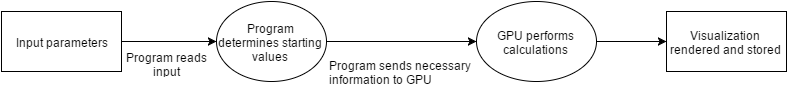
\includegraphics[width=\textwidth]{WorkContextDiagram} 
\end{figure} 

\subsubsection{Work Partitioning}
All tasks will be divided equally among all members of the development team. The team will work together to initially define the interface for using the GPU to run calculations, and once that is completed each member will independently work on porting specific classes to the GPU. Testing will be done throughout the development by the developers. This ensures that all developers are able to easily debug their contributions.

% ----------------------------- Sub Section ----------------------------- %
\subsection{Business Data Model \& Data Dictionary} % Rob
NA -- The product does not store any data, and requires no data model.

% ----------------------------- Sub Section ----------------------------- %
\subsection{The Scope of the Product}
The following table outlines the use cases for the product.

\begin{table}[h]
\centering
\caption{Product Use Cases Summary}
\begin{tabularx}{\textwidth}{c|l|l|X}
\Xhline{2\arrayrulewidth}
\bf PUC \# & \bf PUC Name & Actor(s) & \bf Input/Output\\
\hline
\ref{PUC_SimulatingParticles} & Simulating Particles & Researcher & Simulation parameters (in), Distribution of particle's locations (out)\\
\Xhline{2\arrayrulewidth}
\end{tabularx}
\end{table}

Descriptions of each PUC, referenced by PUC \# are as follows.
\begin{enumerate}
\item \label{PUC_SimulatingParticles} The software will be used by researchers wishing to simulate large numbers of particles interactions with materials. The researcher sets simulation parameters, including the number of particles, their lifetime, and the material properties before running the simulation. On completion, the program gives back a map of where each particle traveled, so researchers can study where the particles are most probably to end up.
\end{enumerate}

% ----------------------------- Sub Section ----------------------------- %
\subsection{Functional Requirements} \label{ReqType_Functional}
\requirement
{Req_RunGPU}
{ReqType_Functional}
{PUC_SimulatingParticles}
{Particle computations run on the GPU}
{Design requirement, will allow particle simulations to run faster (requirement \ref{Req_SpeedLatency})}
{Running the product with GPU computation enabled will result in all computations on particles being offloaded from the CPU (existing product) to the GPU (new product)}
{Very High}
{Created September 29, 2015}
\\\\

\requirement
{Req_EasyChange}
{ReqType_Functional}
{PUC_SimulatingParticles}
{Changing existing projects to run with new GPU functions should be easy}
{Design requirement, the user is able to easily choose to run old or new projects on the GPU.}
{User should be able to quickly enable GPU computations after referencing the documentation. If their hardware is compatible, their project should run with no errors.}
{High}
{Created September 29, 2015}
\\\\

\requirement
{Req_NoChangeOld}
{ReqType_Functional}
{PUC_SimulatingParticles}
{Existing projects should not be affected by the new code. By default, they will continue to run on the CPU.}
{Design Requirement, need to ensure that users can continue to use GEANT-4 as before.}
{Running an existing simulation should execute on the CPU by default as before with no performance regressions and identical results.}
{High}
{Created September 29, 2015}
\\\\

\requirement
{Req_CompatableGPU}
{ReqType_Functional}
{PUC_SimulatingParticles}
{Trying to run the simulation on the GPU with a computer that does not have a compatible graphics card should be detected and cause it to run on CPU like before.}
{New product should not limit the amount of users who can use GEANT-4}
{Any computer that can currently run the existing product should be able to run the new product.}
{Medium}
{Created September 29, 2015}

% ----------------------------- Sub Section ----------------------------- %
\subsection{Look and Feel Requirements}\label{ReqType_Look} % Victor
\subsubsection{Appearance Requirements}
NA -- The scope of the project does not include any visual aspects. Simulations are run through the command line.

\subsubsection{Style Requirements} 
\requirement
{Req_CodeOrganization}
{ReqType_Look}
{PUC_SimulatingParticles}
{The code should be well organized and appear readable to any who might want to edit it.}
{Revised code should not inhibit the modifying or understanding of G4-STORK}
{Any persons with an understanding of the existing project should be able to clearly understand the modified code.}
{Medium}
{Created October 6, 2015}

% ----------------------------- Sub Section ----------------------------- %
\subsection{Usability and Humanity Requirements}\label{ReqType_Usabil} % Rob

\subsubsection{Ease of Use Requirements}
\requirement
{Req_Ease of Use}
{ReqType_Usabil}
{PUC_SimulatingParticles}
{The functionality and procedures involved should be manageable for a university undergraduate (or higher) with experience in quantum mechanics, linear algebra, and computer programming.}
{The software is extremely technical, and requires exposure and understanding to quantum physics and computer programming.}
{Any given McMaster undergrad with experience in quantum mechanics, linear algebra, and computer programming should be able to learn to use the software.}
{Medium}
{Created October 6, 2015}

\subsubsection{Personalization and Internationalization Requirements}
\requirement
{Req_Personalization and Internationalization}
{ReqType_Usabil}
{PUC_SimulatingParticles}
{There will be no adjustments for personal and international preferences offered.}
{The software follows a rigerous scientific standard.}
{A given user with personal (non-technical) barriers to achieving complete satisfaction with the software will be responsible for overcoming such barriers.}
{Medium}
{Created October 6, 2015}

\subsubsection{Learning Requirements}
\requirement
{Req_Learning}
{ReqType_Usabil}
{PUC_SimulatingParticles}
{Utilization of the software should be learnable given 2-3 weeks of training.}
{Although the prerequisite knowledge assumed of the user is massive, the learning curve for such a person is not.}
{Any university undergraduate student with solid foundations in quantum mechanics and computer programming should be able to learn to operate the software in roughly 2 or 3 weeks.}
{Medium}
{Created October 6, 2015}

\subsubsection{Understandability and Politeness Requirements}
NA\\

\subsubsection{Accessibility Requirements}
\requirement
{Req_Accessibility}
{ReqType_Usabil}
{PUC_SimulatingParticles}
{The software should be accessible to any person who can learn and use a shell based operating system.}
{Vision/reading/typing is required for the operation of the software, and there will be no accessibility alternatives offered.}
{A blind university student who potentially has trouble using a shell based operating system may have trouble with the software.}
{Medium}
{Created October 6, 2015}

% ----------------------------- Sub Section ----------------------------- %
\subsection{Performance Requirements}\label{ReqType_Performance}
\subsubsection{Speed and Latency Requirements}
\requirement
{Req_SpeedLatency}
{ReqType_Performance}
{PUC_SimulatingParticles}
{Decrease the time it takes to run a particle simulation while maintaining the same output.}
{The entire purpose of the project is to improve the speed of the simulation.}
{Running a simulation with a given set of input parameters should complete significantly faster on the product as compared to the existing software. Both should have identical outputs.}
{Very High}
{Created September 27, 2015}

\subsubsection{Safety Critical Requirements}
NA -- The software is not used in safety critical environments. It is a tool for researchers to study particle interactions.

\subsubsection{Precision of Accuracy Requirements}
\requirement
{Req_Precision}
{ReqType_Performance}
{PUC_SimulatingParticles}
{Results should have same accuracy whether simulation is run on CPU or GPU.}
{If results are not as accurate as with the existing product then researchers will not be able to draw as strong conclusions.}
{The results of a simulation should be identical on the new product as the existing one, given that the inputs are the same.}
{High}
{Created September 27, 2015}

\subsubsection{Reliability and Availability Requirements}
\requirement
{Req_Reliability}
{ReqType_Performance}
{PUC_SimulatingParticles}
{The product should be at least as stable as the existing product.}
{Researchers require an extremely stable product, we do not want to introduce any new crashes or bugs.}
{Testing the product with a variety of simulations should never result in a crash.}
{High}
{Created September 27, 2015}

\subsubsection{Robustness or Fault-Tolerance Requirements}
NA -- The product does not need to maintain standards during an unforseen event. It does not handle any sensitive data, and is not constantly required to be running by its users.

\subsubsection{Capacity Requirements}
\requirement
{Req_Capacity}
{ReqType_Performance}
{PUC_SimulatingParticles}
{Due to speed improvements (requirement \ref{Req_SpeedLatency}) a larger number of particles should be able to be simulated in the same period of time.}
{Increasing the number of particles in the simulation will allow researchers to better simulate real-world interactions.}
{A simulation running on the new product will be able to simulate a significantly larger number of particles in the same time as the same simulation on the existing product.}
{High}
{Created September 27, 2015}

\subsubsection{Scalability Requirements}
NA -- The product will be used by single researchers, and is run locally on their machines.

\subsubsection{Longevity Requirements}
NA -- The product is to be completed by April 2016, and there are no plans to extend that lifetime.

% ----------------------------- Sub Section ----------------------------- %
\subsection{Operational and Environmental Requirements}\label{ReqType_Enviro} % Matt

\subsubsection{Expected Physical Environment}
\requirement
{Req_PhysEnviro}
{ReqType_Enviro}
{PUC_SimulatingParticles}
{The product shall be used by an Engineering Physics professor, researcher or student who will be sitting down in a temperature controlled environment.}
{The product should typically only be used in an office environment.}
{95\% of all uses of the product will be used by Engineering Physics professors, researchers or students in sitting down in temperature controlled environments.}
{Low}
{Created October 4, 2015}

\subsubsection{Requirements for interfacing with adjacent Systems}
\requirement
{Req_BackwardsCompatible}
{ReqType_Enviro}
{PUC_SimulatingParticles}
{The product shall work with the last four versions of GEANT-4}
{Backwards compatibility is a nice thing to have.}
{At least the last four versions of GEANT-4 will be able to run this product.}
{Low}
{Created October 4, 2015}

\subsubsection{Productization Requirements}
\requirement
{Req_Distro}
{ReqType_Enviro}
{PUC_SimulatingParticles}
{The product will available on a public repository along with clear instructions for installation}
{Want to make the product easily available}
{90\% of users should be able to acquire the product with out much trouble}
{Low}
{Created October 4, 2015}

\subsubsection{Release Requirements}
\requirement
{Req_Release}
{ReqType_Enviro}
{PUC_SimulatingParticles}
{New versions of the product that have been patched will be available on the public repository and shall not cause previous features to fail.}
{Users should be encouraged to use the latest patch, and should be confident that updating won't negatively impact their work}
{Each new patch of the product will not cause any previous features to fail.}
{Medium}
{Created October 4, 2015}

% ----------------------------- Sub Section ----------------------------- %
\subsection{Maintainability and Support Requirements} % Victor

% ----------------------------- Sub Section ----------------------------- %
\subsection{Security Requirements}\label{ReqType_Security} % Rob
\subsubsection{Access Requirements}
\requirement
{Req_Access}
{ReqType_Security}
{PUC_SimulatingParticles}
{All users have access to all aspects of the product.}
{The product will be open-source.}
{Any user should never fail to access some functionality of the product.}
{High}
{Created October 6, 2015}

\subsubsection{Integrity Requirements}
\requirement
{Req_Integrity}
{ReqType_Security}
{PUC_SimulatingParticles}
{There will be no compromise on the integrity of data outside of physical hardware malfunctions.}
{All data is stored locally and unaltered.}
{A user upon gathering input or output data should never find that their data has been compromised.}
{High}
{Created October 6, 2015}

\subsubsection{Privacy Requirements}
\requirement
{Req_Privacy}
{ReqType_Security}
{PUC_SimulatingParticles}
{The privacy of the data will be managed entirely by and at the discretion of the user.}
{The data is stored and manipulated entirely locally.}
{No user will ever find that their data has been shared without their discretion.}
{High}
{Created October 6, 2015}

\subsubsection{Audit Requirements}

\subsubsection{Immunity Requirements}
\requirement
{Req_Immunity}
{ReqType_Security}
{PUC_SimulatingParticles}
{There will be no specific features to ensure immunity.}
{The only impact external software can have on the program is a cut in performance.}
{The user will be held responsible for ensuring that no external software is hogging the resources required for the project to run at optimal performance.}
{Medium}
{Created October 6, 2015}

% ----------------------------- Sub Section ----------------------------- %
\subsection{Cultural Requirements} % Stuart
NA -- The product is intended for a small number of stakeholders. All content is objective and scientific.

% ----------------------------- Sub Section ----------------------------- %
\subsection{Legal Requirements} % Matt
\subsubsection{Compliance Requirements}
NA -- The product does not store or access any user information. It does not need to comply with any legal standards.

\subsubsection{Standards Requirements}
NA -- There are no internal standards that are required to be met by the product.

% =============================== Section =============================== %
\section{Project Issues}

% ----------------------------- Sub Section ----------------------------- %
\subsection{Open Issues} % Victor

% ----------------------------- Sub Section ----------------------------- %
\subsection{Off-the-Shelf Solutions} % Rob

\subsubsection{Ready-Made Products}
No fully-fledged solution to the given problem has been implemented and distributed. There have been attempts, however, to solving certain portions of the problem. At the Helsinki Institute of Physics (HIP) a team of three attempted to test the potential efficiency increase of porting GEANT-4 code to a GPU. They ported some small portions of GEANT-4, but determined that taking on the entire project would be difficult. Their conclusions supported the conjecture that running the code on a GPU would offer significant increases in performance.

\subsubsection{Reusable Components}
Although there is not any hard-copy code that can be reused, the team of three from HIP have published a research paper that may be used as a starting point for the current project.

\subsubsection{Products That Can Be Copied}
NA -- There are no existing products that can be copied.

% ----------------------------- Sub Section ----------------------------- %
\subsection{New Problems}\label{SubSec_NewProbs} % Stuart
\subsubsection{Effects on the Current Environment}
The new product will be designed as an opt-in addition to the existing product. That is, unless manually changed by the user, the program will execute identically as before, running on the CPU. The motivation for this is to ensure compatibility, as the programming environment for GP-GPU programming is restricted to certain hardware. The current environment will not be affected by the changes unless the user specifically decides to use them.

\subsubsection{Effects on the Installed Systems}
Requirement \ref{Req_EasyChange} specifies the importance of creating a simple interface for the user to enable the changes in the new system, or revert to the previous one. Changes to the code will be isolated, and only used when they are manually enabled.

\subsubsection{Potential User Problems}
Due to the separation of the changes and the existing product, users will not negatively respond to the changes, indeed they won't even notice them unless actively looking. To use the new product's features, users will enable them and then execute the program in an identical manner to how the existing software works (requirement \ref{Req_EasyChange}).

\subsubsection{Limitations of the Anticipated Implementation Environment That May Inhibit the New Product}
To run the GP-GPU computations, specific hardware is required (recent NVIDIA graphics card).

\subsubsection{Follow-Up Problems}
There are a number of potential situations that could lead to the product failing. We are confident that we will be able to succeed, however we realize that there is a possibility of failure, and have outlined the potential causes below.
\begin{itemize}
\item Learning curve for existing G4-STORK codebase is too steep, cannot gain adequate understanding to implement changes in time constraints
\item Porting existing algorithms to CUDA requires too much work, and we are not able to run the algorithms on a GPU within time constraints
\item The current product's interface for the specific algorithms that will be ported is not well-enough defined
\item The large models used in the simulation exceed memory limitations on the GPU, and cannot be run on existing hardware
\item Performance gains from the GPU are negligible, due to the structure of the computations
\item Numerical accuracy problems lead to different results from simulations run on the existing product vs. the new product
\end{itemize}

% ----------------------------- Sub Section ----------------------------- %
\subsection{Tasks}\label{SubSec_Tasks} % Matt
Record of Proposed Project \hfill September 18\\
Problem Statement \hfill September 25\\
Requirements Document Revision 0 \hfill October 9\\
Proof of Concept Plan \hfill October 23\\
Test Plan Revision 0 \hfill October 30\\
Proof of Concept Demonstration \hfill November 16 - 27\\
Design Document Revision 0 \hfill January 1\\
Revision 0 Demonstration \hfill February 1 - 27\\
User's Guide Revision 0 \hfill February 29\\
Test Report Revision 0 \hfill March 21\\
Final Demonstration (Revision 1) \hfill Exam period\\
Final Documentation (Revision 1) \hfill April 1

% ----------------------------- Sub Section ----------------------------- %
\subsection{Migration to the New Product} % Victor

% ----------------------------- Sub Section ----------------------------- %
\subsection{Risks} % Rob

Because our software has research based aspirations and goals, some traditional risks are less catastrophic to the success of the project, but are still risks nonetheless. The following may pose to be potential risks:\\

\begin{itemize}
	\item Excessive schedule pressure
	\item Technical/Resource limitations
	\item Inadequate measurements
	\item Optimistic time constraints
\end{itemize}

% ----------------------------- Sub Section ----------------------------- %
\subsection{Costs} % Stuart
All software used in the project is open-source and/or available for free. Existing hardware will be used for development, so there are no associated monetary costs.\\

We have very clear and well-defined deadlines for each deliverable, and are in full confidence that we will meet each one. The time it takes for each deliverable will be variable, but the date of completion for each is concrete, as outlined in \ref{SubSec_Tasks}.

% ----------------------------- Sub Section ----------------------------- %
\subsection{User Documentation and Training} % Matt
\begin{itemize}
	\item Function descriptions shall be provided for every new function in the code
	\item There shall be a thorough Readme file accompanying the project that will explain to the user the changes as well as how to enable GPU computation
	\item Users who know how to use G4-STORK should be able to easily run it on the GPU
\end{itemize}

% ----------------------------- Sub Section ----------------------------- %
\subsection{Waiting Room} % Victor
There are currently no plans for extended requirements for future releases.

% ----------------------------- Sub Section ----------------------------- %
\subsection{Ideas for Solutions} % Rob
Some solutions to a few potential problems have been breifly mentioned in the above section (see \ref{SubSec_NewProbs}). Outside of those, we can resolve usability issues with a well-written user manual, which will explain how to download the software (or for previous GEANT4 users, how to upgrade). We can also provide documentation which can distinguish if a certain user's machine is eligible for the software. \\
Additionally, in terms of organizational and production problems that may arise, we will schedule meetings with both our group and our supervisors. We can utilize well known software development procedures (such as an Agile strategy) to ease the managerial work required for development of the product to run smoothly.\\

\end{document}
